\documentclass[article,A4,12pt]{llncs}

% Conditional compilation.
% NOTE: If you set fullversionfalse, just compile ONCE so that TOC stays unchanged.
\newif\iffullversion
\fullversiontrue
%\fullversionfalse

\usepackage[T1]{fontenc}
\usepackage{amsmath}
\usepackage{amssymb}
\usepackage{amsfonts}
\usepackage{mathrsfs, bm}

\usepackage{graphicx}
\usepackage{tabularx}
\usepackage{subfig}
\usepackage{epsf,times}
\usepackage{color}
\usepackage{wrapfig}
\usepackage{cases}
\usepackage{multicol}

\usepackage[T1]{fontenc}
%\newcommand{\tmname}[1]{\textsc{#1}}
%\newcommand{\tmop}[1]{\ensuremath{\operatorname{#1}}}
%\newcommand{\tmsamp}[1]{\textsf{#1}}
%\newcommand{\tmtextsc}[1]{{\scshape{#1}}}
%\newcommand{\tmtextsl}[1]{{\slshape{#1}}}
%\newcommand{\tmtexttt}[1]{{\ttfamily{#1}}}

\leftmargin=0.0cm
\oddsidemargin=0.5cm
\evensidemargin=0.5cm
\topmargin=0cm
\textwidth=16.0cm
%\textheight=21.5cm
\textheight=20.0cm
\pagestyle{plain}
\setlength{\columnsep}{20pt}

\def\m{\mathbf{m}}
\def\H{\mathbf{H}}
\def\E{\mathbf{E}}
\newcommand{\vepsi}{{\varepsilon}}
\def\hnorm#1#2{\vert\,#1\,\vert_{#2}}
\newcommand{\R}{{\mathbb R}}
\newcommand{\Sph}{{\mathbb S}}
\def\x{\mathbf{x}}
\def\hvec{\overline{\mathbf{h}}}
\def\evec{\overline{\mathbf{e}}}

\newcommand{ \etal}{\mbox{\emph{et al. }}}

\newcommand\vect[1]{\mbf{#1}}
\newcommand{\mbf}[1]{\mbox{\boldmath$#1$}} 
\newcommand{\RC}[1]{#1 $\times$ #1 $\times$ #1}
\def\um{$\mu$m}
\def\C{$^{\circ}\mathrm{C}$}

\newcommand{\Rmnum}[1]{\expandafter\@slowromancap\romannumeral #1@}

% DEFINITION OF CUSTOM FONT SIZE
\newcommand{\customfontA}{\fontsize{50}{55}\selectfont}
\newcommand{\customfontB}{\fontsize{14.4}{20}\selectfont}
\newcommand{\customfontC}{\fontsize{30}{35}\selectfont}

\DeclareMathAlphabet{\mathpzc}{OT1}{pzc}{m}{it}

\def\clovek#1{\noindent\bgroup\vbox{\noindent#1}\egroup\vskip1em}



\begin{document}



%%%%%%%%%%%%%%%%%%%%%%%%%%%%%%%%%%%%%%%%%%%%%%%%%%%%%%%%%%%%%%%%%%%%%%%%%

\pagestyle{empty}

\vbox{}
\begin{figure}[!ht]
%\hspace{-4mm}

\includegraphics[width=8cm]{imgp/logo.png}
\vspace{18mm}
\end{figure}
\vbox{}
\vspace{0.5cm}


\begin{figure}[!ht]
\begin{center}
\vspace{-6mm}
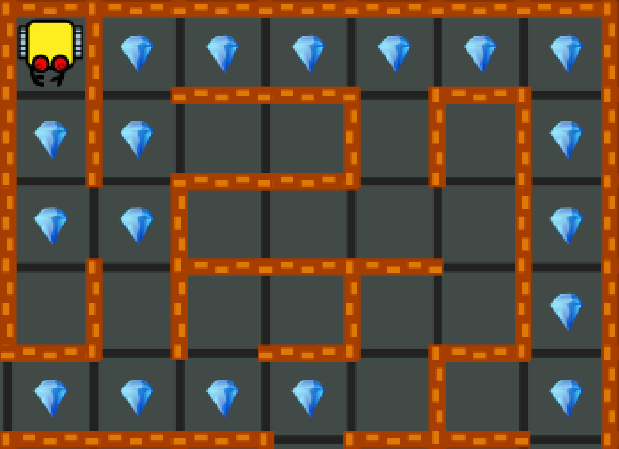
\includegraphics[width=0.26\textheight]{imgk/karel-logo.png}\ \ \ \ \ \ 

\includegraphics[width=0.2\textheight]{imgp/python-logo.png}
\vbox{}
\vspace{-9mm}
\end{center}
\end{figure}
\begin{center}
\vspace{2.8cm}
{\huge \bf Review Questions}
\end{center}
\vbox{}
\begin{center}
\iffullversion
\else
\vspace{2mm}
\centerline{\huge \color{red}{PREVIEW}}
\fi
\vfill
{\large
{\bf Pavel Solin}, University of Nevada, Reno\\
{\bf Salih Dede}, Coral Academy of Science, Reno
}
\end{center}
\newpage
\vbox{}
\vfill
\begin{center}
{
The textbook {\em Intro to Programming with Karel the Robot and Python} that 
comprises this Review Book
can be ordered at {\tt http://introtoprogramming.net}. The textbook 
is also available as part of the NCLab course {\em Intro to Programming} 
that can be purchased at {\tt http://introtoprogramming.net}.
Unauthorized copying and sharing is prohibited.
}
\vfill

Copyright 2012 FEMhub Inc. All rights reserved.
\end{center}




\section*{}
\small

\normalsize

\newpage
%{\ }
\setcounter{tocdepth}{2}
\tableofcontents
%\pagestyle{plain}

\newpage

\pagestyle{plain}
\setcounter{page}{1}

%%%%%%%%%%%%%%%%%%%%%%%%%%%%%%%%%%%%%%%%%%%%%%%%%%%%%%%%%%%%%%%%%%%%%%%%%

\part{Karel the Robot}

\section{Introduction}

For all review questions in this book: None, one, or multiple
choices may be correct.

\begin{enumerate}
\item Name the university where Karel the Robot was created.
\begin{enumerate}
\item[A1] MIT
\item[A2] Princeton
\item[A3] Harvard
\item[A4] Stanford
\end{enumerate}
  \begin{itemize}
    \item A4
  \end{itemize}
\item What is the programming language that you should learn after Karel?
\begin{enumerate}
\item[A1] C
\item[A2] Python
\item[A3] Haskell
\item[A4] Fortran
\end{enumerate}
  \begin{itemize}
    \item A2
  \end{itemize}
\item What is the biggest conceptual difference between Karel and standard
      procedural programming languages such as Python, C, C++ or Fortran?
\begin{enumerate}
\item[A1] Karel only knows five commands.
\item[A2] Karel only can do simple algorithms.
\item[A3] Karel does not know math.
\item[A4] Karel has only five sensors.
\end{enumerate}
  \begin{itemize}
    \item A3
  \end{itemize}
\item Where does Karel live and what objects does he like to collect?
\begin{enumerate}
\item[A1] Karel lives in a maze and he likes to collect gems.
\item[A2] Karel lives in a cave and he likes to collect gold nuggets.
\item[A3] Karel lives on an island and he likes to collect coconuts.
\item[A4] Karel lives in a marketplace and he likes to collect coins from the ground.
\end{enumerate}
  \begin{itemize}
    \item A1
  \end{itemize}
\item What is the command that moves the robot one step forward?
\begin{enumerate}
\item[A1] step
\item[A2] forward
\item[A3] go
\item[A4] move
\end{enumerate}
  \begin{itemize}
    \item A3
  \end{itemize}
\item What is the command that turns the robot to the left?
\begin{enumerate}
\item[A1] left\_turn
\item[A2] turn\_left
\item[A3] turnleft
\item[A4] left
\end{enumerate}
  \begin{itemize}
    \item A4
  \end{itemize}
\item What is the command that turns the robot to the right?
\begin{enumerate}
\item[A1] right\_turn
\item[A2] right
\item[A3] turnright
\item[A4] turn\_right
\end{enumerate}
  \begin{itemize}
    \item A2
  \end{itemize}
\item What is the command to pick up a gem from the ground?
\begin{enumerate}
\item[A1] pick
\item[A2] pick\_gem
\item[A3] get
\item[A4] get\_gem
\end{enumerate}
  \begin{itemize}
    \item A3
  \end{itemize}
\item What is the command to drop a gem on the ground?
\begin{enumerate}
\item[A1] put
\item[A2] drop\_gem
\item[A3] drop 
\item[A4] put\_gem
\end{enumerate}
  \begin{itemize}
    \item A1
  \end{itemize}
\item What sensor helps the robot avoid crashing into walls?
\begin{enumerate}
\item[A1] wall\_ahead
\item[A2] wall
\item[A3] crash
\item[A4] danger
\end{enumerate}
  \begin{itemize}
    \item A2
  \end{itemize}
\item What sensor helps the robot detect gems?
\begin{enumerate}
\item[A1] detect\_gem
\item[A2] see\_gem
\item[A3] gem
\item[A4] near\_gem
\end{enumerate}
  \begin{itemize}
    \item A3
  \end{itemize}
\item What sensor does the robot use to check whether he has any gems in his bag?
\begin{enumerate}
\item[A1] bag\_full
\item[A2] bag\_empty
\item[A3] has\_gems
\item[A4] empty
\end{enumerate}
  \begin{itemize}
    \item A4
  \end{itemize}
\item What sensor helps the robot detect his orientation?
\begin{enumerate}
\item[A1] south
\item[A2] north
\item[A3] east
\item[A4] west
\end{enumerate}
  \begin{itemize}
    \item A2
  \end{itemize}
\item What sensor helps the robot detect whether he is at home?
\begin{enumerate}
\item[A1] at\_home
\item[A2] finished
\item[A3] home
\item[A4] stop
\end{enumerate}
  \begin{itemize}
    \item A3
  \end{itemize}
\item What is the most important skill in computer programming?
\begin{enumerate}
\item[A1] Writing short programs.
\item[A2] Designing great algorithms.
\item[A3] Writing programs quickly.
\item[A4] Knowing many programming languages.
\end{enumerate}
  \begin{itemize}
    \item A2
  \end{itemize}
\end{enumerate}

\section{Launching Karel}

\begin{enumerate}
\item What can you do with displayed Karel projects that you clone into your account?
\begin{enumerate}
\item[A1] View but not run.
\item[A2] View and run but not edit.
\item[A3] View, run and edit but not save.
\item[A4] View, run, edit, save, whatever, they are all yours!
\end{enumerate}
  \begin{itemize}
    \item A4
  \end{itemize}
\item What are the four modes of the Karel application?
\begin{enumerate}
\item[A1] Clicking, Programming, Designer, Games.
\item[A2] Mode 1, Mode 2, Mode 3, Mode 4.
\item[A3] Beginner mode, Intermediate mode, Advanced mode, Expert mode.
\item[A4] Karel has no modes.
\end{enumerate}
  \begin{itemize}
    \item A1
  \end{itemize}
\item What is the difference between Levels 1 and 2?
\begin{enumerate}
\item[A1] In Level 2 the robot has more sensors. 
\item[A2] In Level 2 one can only guide the robot with the mouse.
\item[A3] In Level 2 one can only use 5 commands.
\item[A4] In Level 2 programs can contain conditions, loops, and custom commands. 
\end{enumerate}
  \begin{itemize}
    \item A4
  \end{itemize}
\item In which level does the user start working with logical and numerical variables?
\begin{enumerate}
\item[A1] Level 1.
\item[A2] Level 2.
\item[A3] Level 3.
\item[A4] Level 4.
\end{enumerate}
  \begin{itemize}
    \item A3
  \end{itemize}
\item What is taught in Level 3?
\begin{enumerate}
\item[A1] Parallel programming.
\item[A2] Object-oriented programming.
\item[A3] Scientific computing.
\item[A4] Numerical and logical variables.
\end{enumerate}
  \begin{itemize}
    \item A4
  \end{itemize}
\item In which mode can the user build custom mazes?
\begin{enumerate}
\item[A1] Clicking.
\item[A2] Programming.
\item[A3] Designer.
\item[A4] Games.
\end{enumerate}
  \begin{itemize}
    \item A3
  \end{itemize}
\end{enumerate}

\section{Clicking Mode}

\begin{enumerate}
\item How can Karel be switched to Clicking?
\begin{enumerate}
\item[A1] Through Settings in main menu.
\item[A2] By pressing the Programming button twice
\item[A3] By pressing the Clicking button.
\item[A4] Through the File menu.
\end{enumerate}
  \begin{itemize}
    \item A3
  \end{itemize}
\item Look at the arrows and decide which direction the robot is facing!
\newpage
\begin{figure}[!ht]
\begin{center}
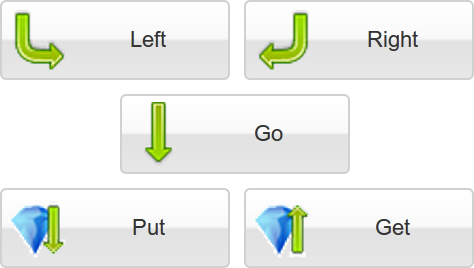
\includegraphics[width=6.2cm]{imgk/buttons-all-3.png}
\end{center}
\end{figure}
\begin{enumerate}
\item[A1] North
\item[A2] South
\item[A3] East
\item[A4] West
\end{enumerate}  
  \begin{itemize}
    \item A2
  \end{itemize}
\item Look at the button and decide which direction the robot is facing!
\begin{figure}[!ht]
\begin{center}
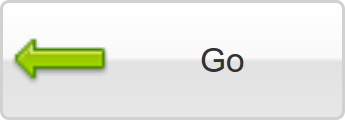
\includegraphics[width=3cm]{imgk/button-go-3.png}
\end{center}
\end{figure}
\begin{enumerate}
\item[A1] North
\item[A2] South
\item[A3] East
\item[A4] West
\end{enumerate}
  \begin{itemize}
    \item A4
  \end{itemize}
\item Which direction is the robot facing after 
this button is pressed?
\begin{figure}[!ht]
\begin{center}

\includegraphics[width=3cm]{imgk/button-left-3.png}
\end{center}
\end{figure}
\begin{enumerate}
\item[A1] North
\item[A2] South
\item[A3] East
\item[A4] West
\end{enumerate}
  \begin{itemize}
    \item A2
  \end{itemize}
\newpage
\item What is the function of the following button?
\begin{figure}[!ht]
\begin{center}
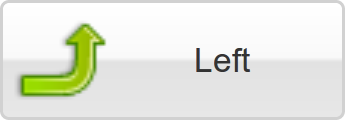
\includegraphics[width=3cm]{imgk/button-left-1.png}
\end{center}
\end{figure}
\begin{enumerate}
\item[A1] Make one step forward, turn left, and make one step forward.
\item[A2] Make one step forward and turn left
\item[A3] Step aside towards East and then make one step forward.
\item[A4] Turn left.
\end{enumerate}
  \begin{itemize}
    \item A4
  \end{itemize}
\item The robot is facing North. Which button will make him face East?
\begin{enumerate}
\item[A1] 
\begin{figure}[!ht]
\begin{center}

\includegraphics[width=3cm]{imgk/button-put-1.png}
\vspace{-10mm}
\end{center}
\end{figure}
\item[A2] 
\begin{figure}[!ht]
\begin{center}
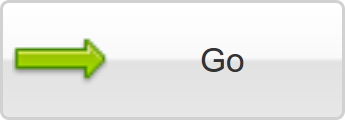
\includegraphics[width=3cm]{imgk/button-go-1.png}
\vspace{-10mm}
\end{center}
\end{figure}
\item[A3] 
\begin{figure}[!ht]
\begin{center}

\includegraphics[width=3cm]{imgk/button-right-2.png}
\vspace{-10mm}
\end{center}
\end{figure}
\item[A4] 
\begin{figure}[!ht]
\begin{center}

\includegraphics[width=3cm]{imgk/button-left-2.png}
\end{center}
\end{figure}
\end{enumerate}
  \begin{itemize}
    \item A3
  \end{itemize}
\item The robot is facing South. Which two buttons you need to press 
to make him move one step ahead and turn East?
\begin{enumerate}
\item[A1] 
\begin{figure}[!ht]
\begin{center}

\includegraphics[width=3cm]{imgk/button-go-4.png}\ \ \

\includegraphics[width=3cm]{imgk/button-left-4.png}
\end{center}
\end{figure}
\newpage
\item[A2] 
\begin{figure}[!ht]
\begin{center}

\includegraphics[width=3cm]{imgk/button-go-4.png}\ \ \

\includegraphics[width=3cm]{imgk/button-right-4.png}
\end{center}
\end{figure}
\item[A3] 
\begin{figure}[!ht]
\begin{center}
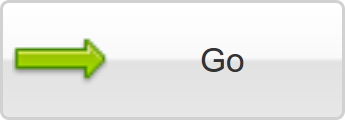
\includegraphics[width=3cm]{imgk/button-go-1.png}\ \ \

\includegraphics[width=3cm]{imgk/button-left-4.png}
\end{center}
\end{figure}
\item[A4] 
\begin{figure}[!ht]
\begin{center}
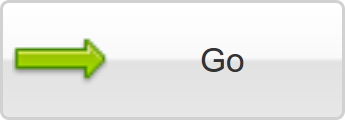
\includegraphics[width=3cm]{imgk/button-go-1.png}\ \ \

\includegraphics[width=3cm]{imgk/button-right-4.png}
\end{center}
\end{figure}
\end{enumerate}
  \begin{itemize}
    \item A1
  \end{itemize}
\item Select one or more correct statements from the four options below!
\begin{figure}[!ht]
\begin{center}
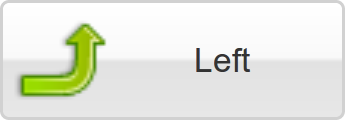
\includegraphics[width=3cm]{imgk/button-left-1.png}\ \ \

\includegraphics[width=3cm]{imgk/button-left-2.png}\ \ \

\includegraphics[width=3cm]{imgk/button-left-3.png}\ \ \

\includegraphics[width=3cm]{imgk/button-left-4.png}
\end{center}
\end{figure}
\begin{enumerate}
\item[A1] All these buttons will turn the robot 90 degrees to the right.
\item[A2] Two of the buttons will turn the robot to the left, the other 
          two will turn him to the right.
\item[A3] The last button on the right will turn the robot to the left.
\item[A4] The last button on the right will turn the robot to the right.
\end{enumerate}
  \begin{itemize}
    \item A3
  \end{itemize}
\item After you press the following button, the robot will:
\begin{figure}[!ht]
\begin{center}

\includegraphics[width=3cm]{imgk/button-right-4.png}
\end{center}
\end{figure}
\begin{enumerate}
\item[A1] Turn left and face West.
\item[A2] Turn right and face West.
\item[A3] Turn right and face East
\item[A4] Turn right and face South.
\end{enumerate}
  \begin{itemize}
    \item A2
  \end{itemize}
\item The robot is facing South. Which two buttons will make him rotate 180 degrees?
\newpage
\begin{enumerate}
\item[A1] 
\begin{figure}[!ht]
\begin{center}

\includegraphics[width=3cm]{imgk/button-left-4.png}\ \ \

\includegraphics[width=3cm]{imgk/button-go-2.png}
\end{center}
\end{figure}
\item[A2] 
\begin{figure}[!ht]
\begin{center}

\includegraphics[width=3cm]{imgk/button-left-4.png}\ \ \
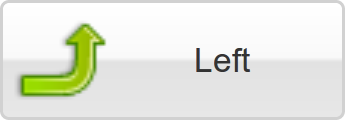
\includegraphics[width=3cm]{imgk/button-left-1.png}
\end{center}
\end{figure}
\item[A3] 
\begin{figure}[!ht]
\begin{center}

\includegraphics[width=3cm]{imgk/button-left-4.png}\ \ \

\includegraphics[width=3cm]{imgk/button-right-4.png}
\end{center}
\end{figure}
\item[A4] 
\begin{figure}[!ht]
\begin{center}
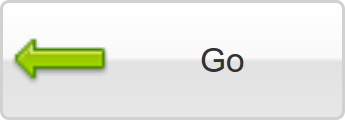
\includegraphics[width=3cm]{imgk/button-go-3.png}\ \ \

\includegraphics[width=3cm]{imgk/button-right-4.png}
\end{center}
\end{figure}
\end{enumerate}
  \begin{itemize}
    \item A2
  \end{itemize}
\end{enumerate}

%%%%%%%%%%%%%%%%%%%%%%%%%%%%%%%%%%%%%%%%%%%%%%%%%%%%%%%%%%%%%%%%%%%%%%%%%%%%

\section{Programming Mode}

\begin{enumerate}
\item Where do we enter programs for Karel?
\begin{enumerate}
\item[A1] In Microsoft Word.
\item[A2] In DreamWeaver.
\item[A3] We upload them from hard disk.
\item[A4] In code cells.
\end{enumerate}
\item Do we have to write one command per line?
\begin{enumerate}
\item[A1] Yes, otherwise the program would not run.
\item[A2] No, but any commands beyond the first are ignored.
\item[A3] No, but doing so makes the code easier to read.
\item[A4] Yes, otherwise the program would not work correctly.
\end{enumerate}
\item The robot's initial situation is as shown in the image. His bag with gems is empty.
\begin{figure}[!ht]
\begin{center}
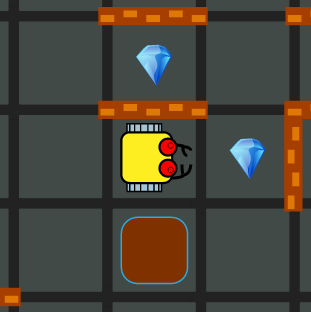
\includegraphics[width=4cm]{imgk/maze-0.png}
\end{center}
\end{figure}
\noindent
Read the following program and select one or more correct statements!
\begin{verbatim}
go
right
get
go
right 
go
\end{verbatim}
\begin{enumerate}
\item[A1] The robot will return home with no gems in the bag.
\item[A2] The robot will return home with one gem in the bag.
\item[A3] The robot will not return home and he will have no gems in the bag.
\item[A4] The robot will not return home and he will have one gem in the bag.
\end{enumerate}
\item The robot's initial situation is the same as in the previous question. He has no gems 
in his bag. Read the following program and select one or more correct statements from the four options below!
\begin{verbatim}
go
get
left
go
left
go
get
right
right
go
right
go
put
go
left 
go
\end{verbatim}
\begin{enumerate}
\item[A1] The robot will return home with two gems in the bag.
\item[A2] The robot will return home with only one gem in the bag.
\item[A3] The robot will not return home and he will have two gems in the bag.
\item[A4] The robot will not return home and he will have only one gem in the bag.
\end{enumerate}
\end{enumerate}

%%%%%%%%%%%%%%%%%%%%%%%%%%%%%%%%%%%%%%%%%%%%%%%%%%%%%%%%%%%%%%%%%%%%%%

\section{Algorithms, Programs, and Bugs}

\begin{enumerate}
\item What is an {\em algorithm}?
\begin{enumerate}
\item[A1] Very short program.
\item[A2] Sequence of instructions for the robot written using the correct commands.
\item[A3] Logical mistake in our program.
\item[A4] Sequence of logical steps leading to the solution of the given task.
\end{enumerate}
\item What is a {\em program}?
\begin{enumerate}
\item[A1] Sequence of logical steps written using human language.
\item[A2] Algorithm that does not contain any mistakes.
\item[A3] Algorithm that is translated from human language to programming language.
\item[A4] Very long algorithm.
\end{enumerate}
\item If the robot does something unexpected, what is the most probable reason for that?
\begin{enumerate}
\item[A1] Something is wrong with the computer.
\item[A2] Internet connection is too slow.
\item[A3] Web browser needs upgrading.
\item[A4] Our algorithm contains a logical mistake.
\end{enumerate}
\item What of the following is a {\em logical} mistake?
\begin{enumerate}
\item[A1] Mistake in an algorithm that causes the robot to do something unexpected.
\item[A2] Opening Karel through the Programming menu instead of through File Manager. 
\item[A3] Typing a command in a wrong way, such as {\tt lft} instead of {\tt left}.
\item[A4] Learning Fortran.
\end{enumerate}
\item What of the following is a {\em syntactical} mistake?
\begin{enumerate}
\item[A1] Writing two commands on the same line.
\item[A2] Having two empty characters between commands.
\item[A3] Mis-spelling a command.  
\item[A4] Mistake that causes the robot to do something unexpected.
\end{enumerate}
\item What of the following will cause an error message?
\begin{enumerate}
\item[A1] Turning the robot four times to the left or right.
\item[A2] Putting two or more gems on each other.
\item[A3] Putting a gem while the bag is empty.
\item[A4] Returning home without any gems.
\end{enumerate}
\item What do we mean by {\em debugging}?
\begin{enumerate}
\item[A1] Apologizing after we ask a friend too many questions.
\item[A2] Playing an algorithm in our head prior to writing a program. 
\item[A3] Looking for mistakes when our program does not work.
\item[A4] Writing a new program after the previous one did not work.
\end{enumerate}
\end{enumerate}

%%%%%%%%%%%%%%%%%%%%%%%%%%%%%%%%%%%%%%%%%%%%%%%%%%%%%%%%%%%%%%%%%%%%%%

\section{Counting Loop}

\begin{enumerate}
\item What command should we use to make the robot repeat something a given number of times?
\begin{enumerate}
\item[A1] {\tt repetition}
\item[A2] {\tt loop}
\item[A3] {\tt for}
\item[A4] {\tt repeat}
\end{enumerate}
\item Why should we always write one command per line?
\begin{enumerate}
\item[A1] To keep the code readable.
\item[A2] To make the code look longer.
\item[A3] Because all programming languages require that.
\item[A4] Because it speeds up communication with server.
\end{enumerate}
\item What is the {\em body} of a {\tt repeat} loop?
\begin{enumerate}
\item[A1] Body of a loop is the number that follows the {\tt repeat} command. 
\item[A2] The command on the first line following the {\tt repeat} command.
\item[A3] One or more commands that follow the {\tt repeat} command and are indented.
\item[A4] One or more commands that follow the {\tt repeat} command and are not indented.
\end{enumerate}
\item Why does the body of a loop need to be indented?
\begin{enumerate}
\item[A1] To make clear where the body of the loop begins and where it ends.
\item[A2] It does not have to be indented, the indentation is optional.
\item[A3] Because the code is visually nicer.
\item[A4] Because the code is easier to read.
\end{enumerate}
\item Which program(s) will rotate Karel 360 degrees?
\begin{enumerate}
\item[A1] 
\begin{verbatim}
 left
 left
 left
 left
\end{verbatim}
\item[A2] 
\begin{verbatim}
 repeat 2
     right
     right
\end{verbatim}
\item[A3] 
\begin{verbatim}
 repeat 4
     left
\end{verbatim}
\item[A4] 
\begin{verbatim}
 repeat 2
     repeat 2
         right
\end{verbatim}
\end{enumerate}
\item Karel needs to pick up 5 gems from the ground, walk 10 steps forward, and put the 5 gems 
      on the ground again. Which one(s) of the following programs will do that?
\begin{enumerate}
\item[A1] 
\begin{verbatim}
 repeat 5
     get
     repeat 10
         go
         repeat 5
             put
\end{verbatim}
\item[A2] 
\begin{verbatim}
 repeat 5
     get
 repeat 10
     go
 repeat 5
     put
\end{verbatim}
\item[A3] 
\begin{verbatim}
 repeat 5
     get
     repeat 10
         go
     repeat 5
         put
\end{verbatim}
\item[A4] 
\begin{verbatim}
 repeat 5
 get
 repeat 10
 go
 repeat 5
 put
\end{verbatim}
\end{enumerate}
\end{enumerate}

%%%%%%%%%%%%%%%%%%%%%%%%%%%%%%%%%%%%%%%%%%%%%%%%%%%%%%%%%%%%%%%%%%%%%%%%%%%%%%%

\newpage
\iffullversion
\else
\vbox{}
\vfill
\pagestyle{empty}
    \begin{center}
    {\huge \color{red}END OF PREVIEW}\\[2cm]

\centerline{\Large Please consider:}
\vspace{1cm}

{\Large \bf Purchasing Online Course with Curriculum}
\vspace{1cm}

    {\Large or,}\\[1cm]

{\Large \bf Ordering Textbook}
\vspace{1cm}

    {\Large Visit {\tt http://introtoprogramming.net}. \\[2cm]
}
\end{center}
{\bf The course includes}:
\begin{itemize}
\item Access to full version of Textbook, Review Book, and Exercise Book.
\item One-click download of interactive review question worksheets.
\item One-click download of interactive programming exercises.
\item One-click distribution to students in your class.
\item One-click collection, automated grading, and progress monitoring.
\item Access to all answers and solution programs.
\end{itemize}

\vfill
    \end{document}
\fi

%%%%%%%%%%%%%%%%%%%%%%%%%%%%%%%%%%%%%%%%%%%%%%%%%%%%%%%%%%%%%%%%%%%%%%

\section{Working with Code and Text Cells}

\begin{enumerate}
\item How can a new text cell be added?
\begin{enumerate}
\item[A1] By clicking on {\tt add} under an existing code cell.
\item[A2] Through {\tt Add new text cell} in the Edit menu.
\item[A3] Through {\tt New} in File menu.
\item[A4] Through {\tt Clone} in File menu.
\end{enumerate}
\item How can we add a new code cell?
\begin{enumerate}
\item[A1] Click on {\tt add} under an existing code cell.
\item[A2] Through {\tt Add new code cell} in the Edit menu.
\item[A3] Through {\tt New} in File menu.
\item[A4] Through {\tt Clone} in File menu.
\end{enumerate}
\item When should we have multiple code cells?
\begin{enumerate}
\item[A1] When our program contains more than one command.
\item[A2] When we want to run parts of the program separately.
\item[A3] When a command is repeated multiple times.
\item[A4] When the program is longer than 10 lines.
\end{enumerate}
\item What is the best way to erase all text from an code cell?
\begin{enumerate}
\item[A1] Close Karel, logout, and login again. 
\item[A2] Restart Karel.
\item[A3] Remove the code cell and add a new one in its place.
\item[A4] Click on {\tt clear} under the code cell.
\end{enumerate}
\item How can a cell be collapsed?
\begin{enumerate}
\item[A1] Click on {\tt remove} under the code cell.
\item[A2] Through {\tt Collapse} in File menu.
\item[A3] Click on the bracket on the right of the cell.
\item[A4] Click on {\tt collapse} under the cell.
\end{enumerate}
\item How can an code cell be removed?
\begin{enumerate}
\item[A1] Click on {\tt add} under the code cell.
\item[A2] Click on {\tt remove} under the code cell.
\item[A3] Click on {\tt clear} under the code cell.
\item[A4] Switch to Designer and back.
\end{enumerate}
\item How can we evaluate all code cells at once?
\begin{enumerate}
\item[A1] Through {\tt Expand all cells} in Edit menu.
\item[A2] Click on the red button in the menu.
\item[A3] Click on {\tt run} under the last code cell.
\item[A4] Click on the green arrow button in the menu.
\end{enumerate}
\item How should running programs be stopped?
\begin{enumerate}
\item[A1] Click on the green arrow button in the menu.
\item[A2] Close the main Karel window.
\item[A3] Click on the red button in the menu.
\item[A4] Click on {\tt stop} under the last code cell.
\end{enumerate}
\item How can we evaluate just one selected code cell?
\begin{enumerate}
\item[A1] Copy and paste the contents of all 
          code cells into the first one, and remove them.
\item[A2] Click on the green arrow button in the menu. 
\item[A3] Click on {\tt run} under the code cell.
\item[A4] Click on {\tt remove} under the code cell.
\end{enumerate}
\end{enumerate}

%%%%%%%%%%%%%%%%%%%%%%%%%%%%%%%%%%%%%%%%%%%%%%%%%%%%%%%%%%%%%%%%%%%%%%

\section{Conditions}

\begin{enumerate}
\item When does the {\tt gem} sensor check true?
\begin{enumerate}
\item[A1] There is at least one gem in the maze.
\item[A2] There is at least one gem in front of the robot.
\item[A3] There are one or more gems under the robot.
\item[A4] The robot's bag contains at least one gem.
\end{enumerate}
\item When does the {\tt North} sensor check true?
\begin{enumerate}
\item[A1] The robot's home is North of him.
\item[A2] The robot is North of his home.
\item[A3] The robot faces South.
\item[A4] The robot faces North.
\end{enumerate}
\item When does the {\tt empty} sensor check true?
\begin{enumerate}
\item[A1] The robot's bag is empty.
\item[A2] There are no gems where the robot stands.
\item[A3] There are no gems in the maze.
\item[A4] There are no gems in the robot's home.
\end{enumerate}
\item When does the {\tt home} sensor check true?
\begin{enumerate}
\item[A1] Robot's home is right in front of the robot.
\item[A2] The robot is in his home.
\item[A3] Robot's home is straight ahead of the robot.
\item[A4] The robot needs to go home to drop all gems that he collected.
\end{enumerate}
\item When does the {\tt wall} sensor check true?
\begin{enumerate}
\item[A1] The robot will reach a wall with one or more steps. 
\item[A2] There is a wall on the robot's right-hand side.
\item[A3] There is a wall right in front of the robot.
\item[A4] There is a wall on the robot's left-hand side.
\end{enumerate}
\item When can Karel see from where he stands whether a wall is two steps ahead?
\begin{enumerate}
\item[A1] Never.
\item[A2] If his home is not in the way.
\item[A3] If no gem is in the way.
\item[A4] If no other wall is in the way.
\end{enumerate}
\item When can the robot check without turning whether a wall is on his right?
\begin{enumerate}
\item[A1] Any time, there is the sensor {\tt right} for that.
\item[A2] Any time, there is the sensor {\tt wall} for that.
\item[A3] Only if he is not at home.
\item[A4] Never.
\end{enumerate}
\item Can Karel check from where he stands whether a gem is one step away?
\begin{enumerate}
\item[A1] Yes, there is the sensor {\tt gem} for that.
\item[A2] No.
\item[A3] Yes but the gem must be in front of him.
\item[A4] Yes but not when he is at home.
\end{enumerate}
\item Can he check from where he stands whether his home is one step away?
\begin{enumerate}
\item[A1] Yes but his home must be in front of him.
\item[A2] Yes, there is the sensor {\tt home} for that.
\item[A3] No.
\item[A4] Yes but not when he is at home.
\end{enumerate}
\item Can the robot check whether he has at least one gem in the bag?
\begin{enumerate}
\item[A1] No.
\item[A2] Yes, he can use the {\tt gem} sensor. 
\item[A3] No, the sensor gem only works for one gem.
\item[A4] Yes, he can use the {\tt empty} sensor.
\end{enumerate}
\item Which program(s) make Karel check whether he stands on a gem, and if so, to pick it up?
\begin{enumerate}
\item[A1] 
\begin{verbatim}
if gem
    get
\end{verbatim}
\item[A2] 
\begin{verbatim}
if not empty
    get
\end{verbatim}
\item[A3] 
\begin{verbatim}
if get
    gem
\end{verbatim}
\item[A4] 
\begin{verbatim}
if empty
    get
\end{verbatim}
\end{enumerate}
\item Which program(s) will turn Karel to the North, regardless the direction he is facing?
\begin{enumerate}
\item[A1] 
\begin{verbatim}
repeat 4
    if not north 
        left
\end{verbatim}
\item[A2] 
\begin{verbatim}
if not north 
    left
else 
    right
\end{verbatim}
\item[A3] 
\begin{verbatim}
if south
    repeat 2
        right
\end{verbatim}
\item[A4] 
\begin{verbatim}
if not north 
    right
\end{verbatim}
\end{enumerate}

\end{enumerate}


%%%%%%%%%%%%%%%%%%%%%%%%%%%%%%%%%%%%%%%%%%%%%%%%%%%%%%%%%%%%%%%%%%%%%%

\section{Conditional Loop}

\begin{enumerate}
\item What is the difference between the {\tt repeat} and {\tt while} loops?
\begin{enumerate}
\item[A1] Body of the {\tt while} loop does not have to be indented.
\item[A2] The {\tt while} loop only can be used when the number of repetitions is known a priori.
\item[A3] The {\tt repeat} loop can do 100 repetitions maximum.
\item[A4] The {\tt repeat} loop only can be used when the number of repetitions is known a priori.
\end{enumerate}
\item Which program will always turn Karel to face West?
\begin{enumerate}
\item[A1] 
\begin{verbatim}
repeat 4
    left
\end{verbatim}
\item[A2] 
\begin{verbatim}
while not west
    right
\end{verbatim}
\item[A3] 
\begin{verbatim}
while not north
    left
left
\end{verbatim}
\item[A4] 
\begin{verbatim}
while not north 
    right
left
\end{verbatim}
\end{enumerate}
\item The maze does not contain any gems and any walls except for the ones that 
      form the outer rectangular boundary.
      The robot stands in the south-west corner facing East. Which program will 
      make the robot walk along the 
      boundary of the maze and bring him back to the original position?
\begin{enumerate}
\item[A1] 
\begin{verbatim}
repeat 4
    while not wall
        go
\end{verbatim}
\item[A2] 
\begin{verbatim}
repeat 4
    while not wall
        go
    left
\end{verbatim}
\item[A3] 
\begin{verbatim}
repeat 4
    while not wall
        go
    right
\end{verbatim}
\item[A4] 
\begin{verbatim}
repeat 4
    while not wall
        left
    go
\end{verbatim}
\end{enumerate}
\end{enumerate}

%%%%%%%%%%%%%%%%%%%%%%%%%%%%%%%%%%%%%%%%%%%%%%%%%%%%%%%%%%%%%%%%%%%%%%

\section{Custom Commands}

\begin{enumerate}
\item Should we, or should we not always try to split a big task into smaller ones?
\begin{enumerate}
\item[A1] No, because the resulting program would be too long.
\item[A2] Yes, because then we can only solve those ones that we like.
\item[A3] Yes, because then we can ask friends to solve some of them for us.
\item[A4] Yes, because the big task becomes simpler to solve.
\end{enumerate}
\item Should we, or should we not replicate computer code?
\begin{enumerate}
\item[A1] Yes, because the resulting program is faster.
\item[A2] Yes, because we do not have to think about new commands.
\item[A3] No, because our code would become prone to errors.
\item[A4] No, because the Karel language does not allow that.
\end{enumerate}
\item When should a new command be defined?
\begin{enumerate}
\item[A1] Whenever the same command is repeated on two consecutive lines in the code.
\item[A2] Whenever the algorithm contains an action that is repeated multiple times
          (a small task inside a big one).
\item[A3] Whenever the code contains an {\tt if - else} statement.
\item[A4] If the code is longer than 100 lines.
\end{enumerate}
\item Which command(s) will empty the robot's bag without causing an error?
\begin{enumerate}
\item[A1] 
\begin{verbatim}
def emptybag
    while gem
        put
\end{verbatim}
\item[A2] 
\begin{verbatim}
def emptybag
    while not gem
        put
\end{verbatim}
\item[A3] 
\begin{verbatim}
def emptybag
    while empty
        put
\end{verbatim}
\item[A4] 
\begin{verbatim}
def emptybag
    while not empty
        put
\end{verbatim}
\end{enumerate}
\item Which command(s) will turn Karel to the South no matter 
      which direction he is facing?
\begin{enumerate}
\item[A1] 
\begin{verbatim}
def turnsouth
    while north
        repeat 2
            left
\end{verbatim}
\item[A2] 
\begin{verbatim}
def turnsouth
    while not north
        repeat 2
            left
\end{verbatim}
\item[A3] 
\begin{verbatim}
def turnsouth
    while not north
        repeat 3
            left
\end{verbatim}
\item[A4] 
\begin{verbatim}
def turnsouth
    while not north
        left
    repeat 2
        left
\end{verbatim}
\end{enumerate}
\end{enumerate}


%%%%%%%%%%%%%%%%%%%%%%%%%%%%%%%%%%%%%%%%%%%%%%%%%%%%%%%%%%%%%%%%%%%%%%

\section{Recursion}

\begin{enumerate}
\item There are three commands {\tt A}, {\tt B}, {\tt C}. Identify all cases of recursion in the four options below!
\begin{enumerate}
\item[A1] {\tt C} calls {\tt B}, {\tt B} calls {\tt A}, {\tt C} calls {\tt A}.
\item[A2] {\tt C} calls {\tt B}, {\tt B} calls {\tt C}, {\tt C} calls {\tt A}.
\item[A3] {\tt C} calls {\tt B}, {\tt B} calls {\tt A}, {\tt A} calls {\tt C}.
\item[A4] {\tt C} calls {\tt B}, {\tt B} calls {\tt A}, {\tt A} calls {\tt B}.
\end{enumerate}
\item What do we mean by {\em base case}?
\begin{enumerate}
\item[A1] The initial state of the robot before executing a recursive program.
\item[A2] Recursion where a single command calls itself directly.
\item[A3] Branch of a conditional statement that makes a recursive call.
\item[A4] Branch of a conditional statement that does not make a recursive call.
\end{enumerate}
\item What happens if base case is not present?
\begin{enumerate}
\item[A1] Recursion turns into an infinite loop.
\item[A2] The program throws an error.
\item[A3] The program will end after the first call to the recursive command.
\item[A4] The program does not throw an error but the robot will do nothing.
\end{enumerate}
\item When should recursion be used?
\begin{enumerate}
\item[A1] The algorithm contains multiple conditional statements.
\item[A2] The algorithm contains multiple repetitions.
\item[A3] After solving part of the problem, the remaining task is similar to the original problem.
\item[A4] Our program contains multiple new commands.
\end{enumerate}
\item Which of the four recursive commands below does the same as this non-recursive one?
\begin{verbatim}
def turn_north
    while not north
        right
\end{verbatim}
\begin{enumerate}
\item[A1]
\begin{verbatim}
def turn_north
    right
    turn_north
\end{verbatim}
\item[A2] 
\begin{verbatim}
def turn_north
    if not north
        right
    turn_north
\end{verbatim}
\item[A3] 
\begin{verbatim}
def turn_north
    if not north
        right
        turn_north
\end{verbatim}
\item[A4] 
\begin{verbatim}
def turn_north
    right
    if not north 
        turn_north
\end{verbatim}
\end{enumerate}
\end{enumerate}

%%%%%%%%%%%%%%%%%%%%%%%%%%%%%%%%%%%%%%%%%%%%%%%%%%%%%%%%%%%%%%%%%%%%%%

\section{Variables}

\begin{enumerate}
\item What are {\em variables} used for in programming? 
\begin{enumerate}
\item[A1] To generate random data.
\item[A2] To make programs shorter.
\item[A3] To store useful information.
\item[A4] To create variable mazes.
\end{enumerate}
\item What values do the variables {\tt gpsx} and {\tt gpsy} have when Karel's
position is as shown in Fig. \ref{fig:var2}?
\newpage
\begin{figure}[!ht]
\begin{center}
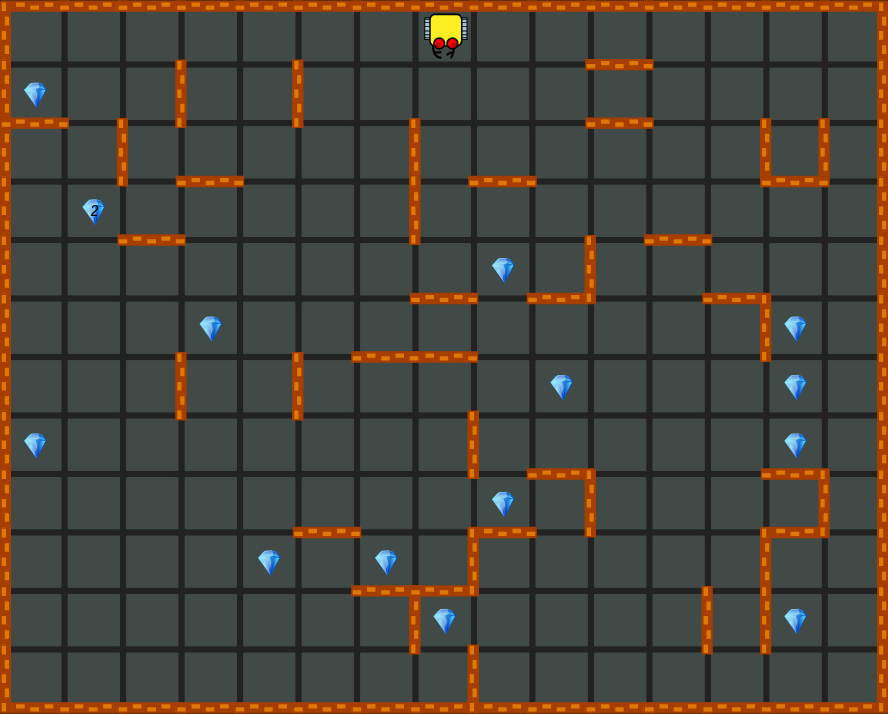
\includegraphics[height=0.4\textwidth]{imgk/variables2.png}
\end{center}
\vspace{-4mm}
\caption{Karel is reading his GPS device again.}
\label{fig:var2}
%\vspace{-1cm}
\end{figure}
\noindent

\begin{enumerate}
\item[A1] {\tt gpsx} is 7 and {\tt gpsy} is 12.
\item[A2] {\tt gpsx} is 8 and {\tt gpsy} is 0.
\item[A3] {\tt gpsx} is 8 and {\tt gpsy} is 12.
\item[A4] {\tt gpsx} is 7 and {\tt gpsy} is 11.
\end{enumerate}
\item What values will the variables {\tt gpsx} and {\tt gpsy} have after
Karel executes the following program? He starts from the position shown 
in Fig. \ref{fig:var2}.
\begin{verbatim}
repeat 5
    while not wall
        go
        if gem
            get
    left
\end{verbatim}
\begin{enumerate}
\item[A1] {\tt gpsx} is 7 and {\tt gpsy} is 7.
\item[A2] {\tt gpsx} is 0 and {\tt gpsy} is 10.
\item[A3] {\tt gpsx} is 9 and {\tt gpsy} is 7.
\item[A4] {\tt gpsx} is 9 and {\tt gpsy} is 11.
\end{enumerate}
\item Which of the following programs are invalid?
\begin{enumerate}
\item[A1] 
\begin{verbatim}
a = gpsx
inc(a)
\end{verbatim}
\item[A2] 
\begin{verbatim}
b = 7
dec(b)
\end{verbatim}
\item[A3] 
\begin{verbatim}
gpsx = 0
inc(gpsx)
\end{verbatim}
\item[A4] 
\begin{verbatim}
e = 1
e = gpsx
e = gpsy
\end{verbatim}
\end{enumerate}
\item Which of the following programs are invalid?
\begin{enumerate}
\item[A1] 
\begin{verbatim}
def count_steps
    n = 0
    while not wall
        go
        inc(n)
    return n
\end{verbatim}
\item[A2] 
\begin{verbatim}
def count_steps
    n = 0
    while not wall
        go
        inc(n, 1)
    print "Number of steps made =", n
\end{verbatim}
\item[A3] 
\begin{verbatim}
def count_steps
    n = 0
    while not wall
        go
        inc(n)
\end{verbatim}
\item[A4] 
\begin{verbatim}
proc count_steps
    while not wall
        go
        inc(n)
    return n
\end{verbatim}
\end{enumerate}
\end{enumerate}

%%%%%%%%%%%%%%%%%%%%%%%%%%%%%%%%%%%%%%%%%%%%%%%%%%%%%%%%%%%%%%%%%%%%%%

\section{Logic}

\begin{enumerate}
\item Let's introduce a variable {\tt my\_age} that stores your age in years.
      This variable is:
\begin{enumerate}
\item[A1] Numerical.
\item[A2] Logical.
\item[A3] Both numerical and logical.
\item[A4] Neither numerical nor logical.
\end{enumerate}
\item What is a {\em logical expression}? 
\begin{enumerate}
\item[A1] Expression that makes sense.
\item[A2] Expression that is always true. 
\item[A3] Expression that is either true or false.
\item[A4] Expression that cannot be false.
\end{enumerate}
\item A is {\tt True} and B is {\tt False}. What is then the value of (A {\em and} {\em not} (A {\em or} B)) ?
\begin{enumerate}
\item[A1] {\tt False}.
\item[A2] {\tt True}.
\item[A3] It can be both {\tt True} and {\tt False}.
\item[A4] Neither {\tt True} nor {\tt False}.
\end{enumerate}
\item A is {\tt True} and B is {\tt True}. What is then the value of (A {\em and} {\em not} (A {\em and} {\em not} B)) ?
\begin{enumerate}
\item[A1] {\tt False}.
\item[A2] {\tt True}.
\item[A3] It can be both {\tt True} and {\tt False}.
\item[A4] Neither {\tt True} nor {\tt False}.
\end{enumerate}
\end{enumerate}

%%%%%%%%%%%%%%%%%%%%%%%%%%%%%%%%%%%%%%%%%%%%%%%%%%%%%%%%%%%%%%%%%%%%%%%%%%%%%%%%%%%%%%%%

\part{Python}

\setcounter{section}{0}
\section{Introduction}

\begin{enumerate}
\item What is the difference between a compiled and a scripting programming language?
\begin{enumerate}
\item[A1] Programs written in compiled languages are binary files. 
\item[A2] Compiled languages are easier to use than the scripting ones.
\item[A3] Programs written in scripting languages are usually more efficient than programs 
          written in the compiled ones.
\item[A4] Scripting languages do not require a compiler.
\end{enumerate}
  \begin{itemize}
    \item A4
  \end{itemize}
\item What languages take better advantage of the underlying hardware architecture
      and why?
\begin{enumerate}
\item[A1] Scripting languages because they are less hardware-dependent.
\item[A2] Compiled languages because the executable files are tailored 
          to the concrete hardware.
\item[A3] Compiled languages because they do not require a linker.
\item[A4] Scripting languages because they do not require a compiler.
\end{enumerate}
  \begin{itemize}
    \item A2
  \end{itemize}
\item Give three examples of compiled programming languages.
\begin{enumerate}
\item[A1] Fortran, C++ and Lua.
\item[A2] Python, Ruby and C.
\item[A3] C, C++ and Fortran.
\item[A4] Python, Lua and Perl.
\end{enumerate}
  \begin{itemize}
    \item A3
  \end{itemize}
\item Give three examples of interpreted programming languages.
\begin{enumerate}
\item[A1] Pascal, Perl and Python.
\item[A2] Lua, C and C++.
\item[A3] Perl, Python and Ruby. 
\item[A4] C, C++ and Fortran.
\end{enumerate}
  \begin{itemize}
    \item A3
  \end{itemize}
\item Where does the name "Python" of the programming language come from?
\begin{enumerate}
\item[A1] The snake, {\em Python regius}.
\item[A2] TV show in Great Britain.
\item[A3] Brand name of remote start systems.
\item[A4] Brand name of aquarium products.
\end{enumerate}
  \begin{itemize}
    \item A2
  \end{itemize}
\item When was the implementation of Python started?
\begin{enumerate}
\item[A1] 1989
\item[A2] 1995
\item[A3] 2000
\item[A4] 2005
\end{enumerate}
  \begin{itemize}
    \item A1
  \end{itemize}
\item Name three programming styles that Python permits.
\begin{enumerate}
\item[A1] Compiled, interpreted, scripting.
\item[A2] Structured, object-oriented, functional.
\item[A3] Procedural, object-oriented, binary.
\item[A4] Compact, literal, extended.
\end{enumerate}
  \begin{itemize}
    \item A2
  \end{itemize}
\item How can displayed Python projects be cloned?
\begin{enumerate}
\item[A1] In Python worksheet through the {\em File} menu.
\item[A2] Through File Manager's {\em Project} menu.
\item[A3] Using the icon {\em Displayed projects} on Desktop.
\item[A4] Python projects cannot be cloned.
\end{enumerate}
  \begin{itemize}
    \item A2
  \end{itemize}
\item How can new Python project be launched?
\begin{enumerate}
\item[A1] Through the {\em Program} menu.
\item[A2] Through File Manager's {\em Settings} menu.
\item[A3] Through File Manager's {\em Project} menu.
\item[A4] Through the Math module.
\end{enumerate}
  \begin{itemize}
    \item A3
  \end{itemize}
\item How are Python programs processed in NCLab?
\begin{enumerate}
\item[A1] They are translated into Javascript and run as a standard web browser application.
\item[A2] They are interpreted on a remote server.
\item[A3] They are interpreted on your PC computer / laptop / tablet.
\item[A4] They are translated into Flash.
\end{enumerate}
  \begin{itemize}
    \item A2
  \end{itemize}
\item What are the types of cells that a Python worksheet can contain?
\begin{enumerate}
\item[A1] Error message cells.
\item[A2] Output cells.
\item[A3] Code cells.
\item[A4] Descriptive text cells.
\end{enumerate}
  \begin{itemize}
    \item A2, A3, A4
  \end{itemize}
\item How can all code cells in a Python worksheet be evaluated at once?
\begin{enumerate}
\item[A1] By typing Evaluate in the last code cell and hitting ENTER.
\item[A2] By clicking on the green arrow under the last code cell.
\item[A3] By clicking on {\em Evaluate all} in the {\em File} menu. 
\item[A4] By clicking on the green arrow button in the main menu.
\end{enumerate}
  \begin{itemize}
    \item A4
  \end{itemize}
\item How can a single code cell be evaluated?
\begin{enumerate}
\item[A1] By clicking on {\tt save} under the code cell.
\item[A2] By clicking on the green arrow button in the menu.
\item[A3] By clicking on the green arrow under the code cell.
\item[A4] By clicking on the red button in the menu.
\end{enumerate}
  \begin{itemize}
    \item A3
  \end{itemize}
\item What is the way to add a new code cell?
\begin{enumerate}
\item[A1] Click on {\tt add} button under a code cell. 
\item[A2] Click on {\em New} in the {\em File} menu.
\item[A3] Click on the larger "A" icon in the menu.
\item[A4] Click on {\em New code cell} in {\em Edit} menu.
\end{enumerate}
  \begin{itemize}
    \item A1
  \end{itemize}
\item How can a new text cell be added?
\begin{enumerate}
\item[A1] Click on {\tt add} button under a code cell. 
\item[A2] Click on {\em New text cell} in the {\em Edit} menu.
\item[A3] Click on {\em New} in the {\em File} menu.
\item[A4] Click on the smaller "A" icon in the menu.
\end{enumerate}
  \begin{itemize}
    \item A1
  \end{itemize}
\item What is the way to remove a code cell or a text cell?
\begin{enumerate}
\item[A1] Click on {\tt remove} button under the cell. 
\item[A2] Click on {\tt clear} under the cell. 
\item[A3] Click on {\em Clear active cell} in the {\em Edit} menu.
\item[A4] Click on {\em Close} in the {\em File} menu.
\end{enumerate}
  \begin{itemize}
    \item A1
  \end{itemize}
\item How can an code cell be evaluated without using the mouse?
\begin{enumerate}
\item[A1] Hold CTRL and press ENTER.
\item[A2] Hold SHIFT and press ENTER.
\item[A3] Press ENTER twice.
\item[A4] Press CTRL + ALT + SHIFT.
\end{enumerate}
  \begin{itemize}
    \item A1, A2
  \end{itemize}
\item Which of the following are scientific libraries for Python?
\begin{enumerate}
\item[A1] GNU Scientific Library.
\item[A2] Numpy.
\item[A3] Scipy.
\item[A4] Sympy.
\end{enumerate}
  \begin{itemize}
    \item A2, A3, A4
  \end{itemize}
\end{enumerate}

%%%%%%%%%%%%%%%%%%%%%%%%%%%%%%%%%%%%%%%%%%%%%%%%%%%%%%%%%%%%%%%%%%%%%

\section{Using Python as a Calculator}

\begin{enumerate}
\item What is the result of $11 / 4$ in Python?
\begin{enumerate}
\item[A1] {\tt 2.75}
\item[A2] {\tt 2}
\item[A3] {\tt 3}
\item[A4] Error message is thrown.
\end{enumerate}
  \begin{itemize}
    \item A2
  \end{itemize}
\item Type $3^2$ using Python syntax:
\begin{enumerate}
\item[A1] {\tt 3\^{}2}
\item[A2] {\tt 3\^{}\^{}2}
\item[A3] {\tt 3*2}
\item[A4] {\tt 3**2}
\end{enumerate}
  \begin{itemize}
    \item A4
  \end{itemize}
\item Type $5$ modulo $2$ using Python syntax:
\begin{enumerate}
\item[A1] {\tt 5 / 2}
\item[A2] {\tt 5 \% 2}
\item[A3] {\tt 5 \& 2}
\item[A4] {\tt 5 \&\& 2}
\end{enumerate}
  \begin{itemize}
    \item A2
  \end{itemize}
\item What is the result of $1**4*2$ in Python?
\begin{enumerate}
\item[A1] {\tt 0}
\item[A2] {\tt 1}
\item[A3] {\tt 2}
\item[A4] {\tt 4}
\end{enumerate}
  \begin{itemize}
    \item A3
  \end{itemize}
\item What do we need to type into an empty Python worksheet in order to evaluate sin($\pi/4$)?
\begin{enumerate}
\item[A1] 
\begin{verbatim}
from numpy import sin
sin(pi/4)
\end{verbatim}
\item[A2] 
\begin{verbatim}
from numpy import sin, pi
sin(pi/4)
\end{verbatim}
\item[A3] 
\begin{verbatim}
from trigonometry import *
sin(pi/4)
\end{verbatim}
\item[A4] 
\begin{verbatim}
from trigonometry import sin, pi
sin(pi/4)
\end{verbatim}
\end{enumerate}
  \begin{itemize}
    \item A2
  \end{itemize}
\item Which of the following are correct ways to define a complex number?
\begin{enumerate}
\item[A1] {\tt 2 + 3j}
\item[A2] {\tt 2 + 3J}
\item[A3] {\tt 2 + 3*j}
\item[A4] {\tt 2 + 3*J}
\end{enumerate}
  \begin{itemize}
    \item A1, A2
  \end{itemize}
\end{enumerate}

%%%%%%%%%%%%%%%%%%%%%%%%%%%%%%%%%%%%%%%%%%%%%%%%%%%%%%%%%%%%%%%%%%%%%

\section{More on Functions}

\begin{enumerate}
\item Why do we define {\em functions} in programming? 
\begin{enumerate}
\item[A1] To isolate self-contained functionality and make it easily reusable.
\item[A2] To make computer programs faster.
\item[A3] To split long programs into multiple segments that have fewer lines.
\item[A4] We should not use functions, it is not a good programming practice.
\end{enumerate}
  \begin{itemize}
    \item A1
  \end{itemize}
\item Which of the following are correct function definitions?
\begin{enumerate}
\item[A1] 
\begin{verbatim}
def subtract(a, b)
    return a - b
\end{verbatim}
\item[A2] 
\begin{verbatim}
def subtract(a, b):
    return a - b
\end{verbatim}
\item[A3] 
\begin{verbatim}
def subtract[a, b]
    return a - b
\end{verbatim}
\item[A4] 
\begin{verbatim}
def subtract(a, b = 5):
    return a - b
\end{verbatim}
\end{enumerate}
  \begin{itemize}
    \item A2, A4
  \end{itemize}
\item When do we have to specify argument types in Python functions?
\begin{enumerate}
\item[A1] Never.
\item[A2] Always.
\item[A3] Always except for numbers and text strings.
\item[A4] Only when default arguments are used.
\end{enumerate}
  \begin{itemize}
    \item A1
  \end{itemize}
\item The modulo operation calculates the 
      rest after integer division. Assume positive integers $a > 0$ and $b > 0$.
      The number $a$ can be decomposed as follows:
      $$
      a = nb + r
      $$  
      where $n \ge 0$ and $0 \le r < b$ are integers.
      Which of the following functions will do the job
      and return the numbers {\tt nb} and {\tt r} ?
\begin{enumerate}
\item[A1] 
\begin{verbatim}
def splitnumber(a, b):
    return a / b, a % b
\end{verbatim}
\item[A2] 
\begin{verbatim}
def splitnumber(a, b):
    return a - a % b, a % b
\end{verbatim}
\item[A3] 
\begin{verbatim}
def splitnumber(a, b):
    n = a / b
    r = a % b
    return n
    return r
\end{verbatim}
\item[A4] 
\begin{verbatim}
def splitnumber(a, b):
    return (a / b) * (a % b), a % b
\end{verbatim}
\end{enumerate}
  \begin{itemize}
    \item A2
  \end{itemize}
\item Of the following four functions, choose the best one to calculate the hypotenuse
      of a right-angled triangle when you know that most of the time one of its shorter
      edges will be 5 cm long.
\begin{enumerate}
\item[A1] 
\begin{verbatim}
from numpy import sqrt
def hypotenuse(a, b):
    return sqrt(a**2 + b**2)
\end{verbatim}
\item[A2] 
\begin{verbatim}
from numpy import sqrt
def hypotenuse(a = 5, b):
    return sqrt(a**2 + b**2)
\end{verbatim}
\item[A3] 
\begin{verbatim}
from numpy import sqrt
def hypotenuse(a, b = 5):
    return sqrt(a**2 + b**2)
\end{verbatim}
\item[A4] 
\begin{verbatim}
from numpy import sqrt
def hypotenuse(a = 5, b = 5):
    return sqrt(a**2 + b**2)
\end{verbatim}
\end{enumerate}
  \begin{itemize}
    \item A3
  \end{itemize}
\end{enumerate}


%%%%%%%%%%%%%%%%%%%%%%%%%%%%%%%%%%%%%%%%%%%%%%%%%%%%%%%%%%%%%%%%%%%%%

\section{Plotting}

\begin{enumerate}
\item Which of the following codes will draw a square with vertices 
[0, 0], [1, 0], [1, 1], [0, 1]?
\begin{enumerate}
\item[A1] 
\begin{verbatim}
from pylab import *
x = [0.0, 1.0, 1.0, 0.0]
y = [0.0, 0.0, 1.0, 1.0]
clf()
plot(x, y)
lab.show()
\end{verbatim}
\item[A2] 
\begin{verbatim}
from pylab import *
x = [0.0, 0.0, 1.0, 1.0]
y = [0.0, 1.0, 1.0, 0.0]
clf()
plot(x, y)
lab.show()
\end{verbatim}
\item[A3] 
\begin{verbatim}
from pylab import *
x = [0.0, 1.0, 1.0, 0.0, 0.0]
y = [0.0, 0.0, 1.0, 1.0, 0.0]
clf()
plot(x, y)
lab.show()
\end{verbatim}
\item[A4] 
\begin{verbatim}
from pylab import *
x = [0.0, 0.0, 1.0, 1.0, 0.0]
y = [0.0, 1.0, 1.0, 0.0, 1.0]
clf()
plot(x, y)
lab.show()
\end{verbatim}
\end{enumerate}
  \begin{itemize}
    \item A3
  \end{itemize}
\item Which of the following codes will plot a cosine function in the interval $(0, \pi)$ using dashed green line with
the step 0.01?
\begin{enumerate}
\item[A1] 
\begin{verbatim}
from numpy import cos, pi
from pylab import *
x = arange(0, pi, 0.01)
y = cos(x)
axis=("equal")
clf()
plot(x, y, 'g-', label="cos(x)")
legend()
lab.show()
\end{verbatim}
\item[A2] 
\begin{verbatim}
from numpy import cos, pi
from pylab import *
x = arange(0, pi, 0.01)
y = cos(x)
clf()
plot(x, y, 'g--')
lab.show()
\end{verbatim}
\item[A3] 
\begin{verbatim}
from numpy import cos, pi
from pylab import *
x = arange(0, pi, 0.05)
y = cos(x)
axis=("equal")
clf()
plot(x, y, 'g--', label="cos(x)")
legend()
lab.show()
\end{verbatim}
\item[A4] 
\begin{verbatim}
from numpy import cos, pi
from pylab import *
x = arange(0, pi, 0.01)
y = cos(x)
axis=("equal")
clf()
plot(x, y, 'g..', label="cos(x)")
legend()
lab.show()
\end{verbatim}
\end{enumerate}
  \begin{itemize}
    \item A2
  \end{itemize}
\end{enumerate}

%%%%%%%%%%%%%%%%%%%%%%%%%%%%%%%%%%%%%%%%%%%%%%%%%%%%%%%%%%%%%%%

\section{More on Variables}

\begin{enumerate}
\item Which of the following Python programs are invalid?
\begin{enumerate}
\item[A1] 
\begin{verbatim}
a = b = 1
\end{verbatim}
\item[A2] 
\begin{verbatim}
a = 1 = b
\end{verbatim}
\item[A3] 
\begin{verbatim}
a = a
\end{verbatim}
\item[A4] 
\begin{verbatim}
a + b = 5
\end{verbatim}
\end{enumerate}
  \begin{itemize}
    \item A2, A3, A4
  \end{itemize}
\item When can a given variable have different types in a Python program?
\begin{enumerate}
\item[A1] Any time.
\item[A2] Never.
\item[A3] Only when variable shadowing takes place.
\item[A4] Only when the types are real number and integer number.
\end{enumerate}
  \begin{itemize}
    \item A1
  \end{itemize}
\item We have two variables {\tt a} and {\tt b} and need to swap their values. Which of the 
following codes will do it?
\begin{enumerate}
\item[A1] 
\begin{verbatim}
a = b = a
\end{verbatim}
\item[A2] 
\begin{verbatim}
a = b
b = a
\end{verbatim}
\item[A3] 
\begin{verbatim}
a = b
c = a
b = a
\end{verbatim}
\item[A4] 
\begin{verbatim}
c = a
a = b
b = c
\end{verbatim}
\end{enumerate}
  \begin{itemize}
    \item A4
  \end{itemize}
\item Should we preferably use local variables, or global variables, and why?
\begin{enumerate}
\item[A1] Global variables because they can be all defined in one place.
\item[A2] Global variables because it yields a faster code.
\item[A3] Local variables because then we can use shadowing.
\item[A4] Local variables because our code is less prone to mistakes. 
\end{enumerate}
  \begin{itemize}
    \item A4
  \end{itemize}
\item Should we use global variables in functions and why?
\begin{enumerate}
\item[A1] Yes, the function definition is simpler.
\item[A2] Yes, the program is less prone to mistakes.
\item[A3] No, it makes the code less transparent and more prone to mistakes.
\item[A4] No, Python does not allow it.
\end{enumerate}
  \begin{itemize}
    \item A3
  \end{itemize}
\item What is shadowing of variables?
\begin{enumerate}
\item[A1] There are two or more functions that all use a local variable of the same name.
\item[A2] The type of a global variable is changed by assigning value of a different type to it. 
\item[A3] The type of a local variable is changed by assigning value of a different type to it. 
\item[A4] There is a local variable whose name matches the name of a global one.
\end{enumerate}
  \begin{itemize}
    \item A4
  \end{itemize}
\end{enumerate}

%%%%%%%%%%%%%%%%%%%%%%%%%%%%%%%%%%%%%%%%%%%%%%%%%%%%%%%%%%%%%%%%%%%%%

\section{Review of Logic}

\begin{enumerate}
\item Let {\tt a} and {\tt b} be Boolean variables. What is the 
result of {\tt (a or b) or (not (a or b))}
\begin{enumerate}
\item[A1] {\tt False}
\item[A2] Undefined.
\item[A3] {\tt False} or {\tt True}, depending on the values of {\tt a} and {\tt b}.
\item[A4] {\tt True}
\end{enumerate}
  \begin{itemize}
    \item A4
  \end{itemize}
\item Let {\tt a} and {\tt b} be Boolean variables. What is the 
result of {\tt (a and b) and (not (a and b))}
\begin{enumerate}
\item[A1] Undefined.
\item[A2] {\tt False} or {\tt True}, depending on the values of {\tt a} and {\tt b}.
\item[A3] {\tt True}
\item[A4] {\tt False}
\end{enumerate}
  \begin{itemize}
    \item A4
  \end{itemize}
\end{enumerate}

%%%%%%%%%%%%%%%%%%%%%%%%%%%%%%%%%%%%%%%%%%%%%%%%%%%%%%%%%%%%%%%%%%%%%

\section{More on Conditions and the {\tt while} Loop}

\begin{enumerate}
\item When should the {\tt elif} statement be used?
\begin{enumerate}
\item[A1] It should not be used as it can be always written using {\tt if - else} statements. 
\item[A2] When there are more than two options in the {\tt if - else} condition. 
\item[A3] When the logical expression in the {\tt if} branch is not likely to be True.
\item[A4] When the logical expression in the {\tt if} branch is likely to be True.
\end{enumerate}
  \begin{itemize}
    \item A2
  \end{itemize}
\item When should the {\tt while} loop be used?
\begin{enumerate}
\item[A1] When we cannot use the {\tt if - else} condition.
\item[A2] When we know exactly how many repetitions there are.
\item[A3] When the loop contains a variable that decreases to zero.
\item[A4] When the number of repetitions is not know a priori.
\end{enumerate}
  \begin{itemize}
    \item A4
  \end{itemize}
\item What is the purpose of the {\tt break} statement?
\begin{enumerate}
\item[A1] Stop the program.
\item[A2] Exit a loop. If multiple loops are embedded, exit all of them.
\item[A3] Exit the body of an {\tt if} or {\tt else} statement.
\item[A4] Exit a loop. If multiple loops are embedded, exit just the closest one.
\end{enumerate}
  \begin{itemize}
    \item A4
  \end{itemize}
\item What will be the output of the following program?
\begin{verbatim}
a = 0
while True:
    a += 1
    if a < 8:
        continue
    print a
    break
\end{verbatim}
\begin{enumerate}
\item[A1] 
\begin{verbatim}
0
1
2
3
4
5
6
7
8
\end{verbatim}
\item[A2] 
\begin{verbatim}
1
2
3
4
5
6
7
8
\end{verbatim}
\item[A3] 
\begin{verbatim}
1
2
3
4
5
6
7
\end{verbatim}
\item[A4] 
\begin{verbatim}
8
\end{verbatim}
\end{enumerate}
  \begin{itemize}
    \item A4
  \end{itemize}
\item What is the Newton's method?
\begin{enumerate}
\item[A1] Method to determine force from mass and gravity.
\item[A2] Method to approximate solutions to nonlinear equations.
\item[A3] Method to calculate Newton integrals.
\item[A4] Method to determine duration of free fall of an apple.
\end{enumerate}
  \begin{itemize}
    \item A2
  \end{itemize}
\end{enumerate}

%%%%%%%%%%%%%%%%%%%%%%%%%%%%%%%%%%%%%%%%%%%%%%%%%%%%%%%%%%%%%%%%%%%%%

\section{Strings}


\begin{enumerate}
\item What of the following are correct ways to include quotes in a string?
\begin{enumerate}
\item[A1] 
\begin{verbatim}
"I say "goodbye", you say "hello""
\end{verbatim}
\item[A2] 
\begin{verbatim}
"I say /"goodbye/", you say /"hello/""
\end{verbatim}
\item[A3] 
\begin{verbatim}
"I say \"goodbye\", you say \"hello\""
\end{verbatim}
\item[A4] 
\begin{verbatim}
"I say \'goodbye\', you say \'hello\'"
\end{verbatim}
\end{enumerate}
  \begin{itemize}
    \item A3, A4
  \end{itemize}
\item What of the following are correct ways to define a multiline string?
\begin{enumerate}
\item[A1] 
\begin{verbatim}
/*
I say "High", you say "Low".
You say "Why?" And I say "I don't know".
*/
\end{verbatim}
\item[A2] 
\begin{verbatim}
"""\
I say "High", you say "Low".
You say "Why?" And I say "I don't know".\
"""
\end{verbatim}
\item[A3] 
\begin{verbatim}
I say "High", you say "Low". \
You say "Why?" And I say "I don't know".
\end{verbatim}
\item[A4] 
\begin{verbatim}
"I say "High", you say "Low". \
You say "Why?" And I say "I don't know"."
\end{verbatim}
\end{enumerate}
  \begin{itemize}
    \item A2
  \end{itemize}
\item What output will be produced by the following code?
\begin{verbatim}
s1 = "Thank you"
s2 = "very"
s3 = "much!"
print s1 + 5*s2 + s3
\end{verbatim}
\begin{enumerate}
\item[A1] 
\begin{verbatim}
Thank you very very very very very much!
\end{verbatim}
\item[A2] 
\begin{verbatim}
Thank youveryveryveryveryverymuch!
\end{verbatim}
\item[A3] 
\begin{verbatim}
Thankyouveryveryveryveryverymuch!
\end{verbatim}
\item[A4] None - an error will be thrown.
\end{enumerate}
  \begin{itemize}
    \item A2
  \end{itemize}
\item What output will be produced by the following code?
\begin{verbatim}
s1 = "intermediate"
s2 = s1[7] + s1[4] + s1[3] + s1[6] + s1[5]
print s2
\end{verbatim}
\begin{enumerate}
\item[A1] 
\begin{verbatim}
dream
\end{verbatim}
\item[A2] 
\begin{verbatim}
dreem
\end{verbatim}
\item[A3] 
\begin{verbatim}
dieta
\end{verbatim}
\item[A4] 
\begin{verbatim}
tamer
\end{verbatim}
\end{enumerate}
  \begin{itemize}
    \item A2
  \end{itemize}
\item What output will be produced by the following code?
\begin{verbatim}
s1 = "intermediate"
s2 = s1[:5]
print s2
s3 = s1[5:10]
print s3
s4 = s1[-2] + s1[-1]
print s4
\end{verbatim}
\begin{enumerate}
\item[A1] 
\begin{verbatim}
intermediate
\end{verbatim}
\item[A2] 
\begin{verbatim}
inter
media
et
\end{verbatim}
\item[A3] 
\begin{verbatim}
inter
media
te
\end{verbatim}
\item[A4] None - an error will be thrown.
\end{enumerate}
  \begin{itemize}
    \item A3
  \end{itemize}
\item What is the correct way to measure and print the length of a string {\tt str}?
\begin{enumerate}
\item[A1] 
\begin{verbatim}
print length(str)
\end{verbatim}
\item[A2] 
\begin{verbatim}
print len(str)
\end{verbatim}
\item[A3] 
\begin{verbatim}
print abs(str)
\end{verbatim}
\item[A4] 
\begin{verbatim}
print str[0]
\end{verbatim}
\end{enumerate}
  \begin{itemize}
    \item A2
  \end{itemize}
\item What will the output of the following code be?
\begin{verbatim}
print range(2, 5)
\end{verbatim}
\begin{enumerate}
\item[A1] 
\begin{verbatim}
[2, 3, 4, 5]
\end{verbatim}
\item[A2] 
\begin{verbatim}
[2, 3, 4, 5, 6]
\end{verbatim}
\item[A3] 
\begin{verbatim}
[2, 3, 4]
\end{verbatim}
\item[A4] 
\begin{verbatim}
[5, 6]
\end{verbatim}
\end{enumerate}
  \begin{itemize}
    \item A3
  \end{itemize}
\item What output corresponds to the following code?
\begin{verbatim}
word = "breakfast"
for m in range(5, 9):
    print word[m]
\end{verbatim}
\begin{enumerate}
\item[A1] 
\begin{verbatim}
fast
\end{verbatim}
\item[A2] 
\begin{verbatim}
kfas
\end{verbatim}
\item[A3] 
\begin{verbatim}
f
a
s
t
\end{verbatim}
\item[A4] 
\begin{verbatim}
kfas
\end{verbatim}
\end{enumerate}
  \begin{itemize}
    \item A3
  \end{itemize}
\end{enumerate}

%%%%%%%%%%%%%%%%%%%%%%%%%%%%%%%%%%%%%%%%%%%%%%%%%%%%%%%%%%%%%%%%%%%%%

\section{Tuples, Lists, and Dictionaries}

\begin{enumerate}
\item What is the variable {\tt var}?
\begin{verbatim}
var = (1, 2, 3, 'A', 'B', 'C', "alpha", "beta", "gamma")
\end{verbatim}
\begin{enumerate}
\item[A1] List.
\item[A2] Tuple.
\item[A3] Dictionary.
\item[A4] None of the above.
\end{enumerate}
  \begin{itemize}
    \item A2
  \end{itemize}
\item What will be the output of the following program?
\begin{verbatim}
var = (1, 2, 3, 'A', 'B', 'C', "alpha", "beta", "gamma")
print var[5]
print var[:3]
print var[6:8]
\end{verbatim}
\begin{enumerate}
\item[A1] 
\begin{verbatim}
B
(1, 2, 3)
('alpha', 'beta', 'gamma')
\end{verbatim}
\item[A2] 
\begin{verbatim}
C
(1, 2, 3)
('alpha', 'beta')
\end{verbatim}
\item[A3] 
\begin{verbatim}
B
(1, 2, 3)
('C', 'alpha', 'beta', 'gamma')
\end{verbatim}
\item[A4]
\begin{verbatim}
B
(1, 2, 3)
('alpha', 'beta')
\end{verbatim}
\end{enumerate}
  \begin{itemize}
    \item A2
  \end{itemize}
\item Can new items be added to a tuple?
\begin{enumerate}
\item[A1] Yes but only to an empty tuple.
\item[A2] Yes but only if all items are of the same type.
\item[A3] No.
\item[A4] Yes but only if not all items are of the same type.
\end{enumerate}
  \begin{itemize}
    \item A3
  \end{itemize}
\item What is the correct way to determine the length of a tuple {\tt T}?
\begin{enumerate}
\item[A1] 
\begin{verbatim}
length(T)
\end{verbatim}
\item[A2] 
\begin{verbatim}
tlength(T)
\end{verbatim}
\item[A3] 
\begin{verbatim}
len(T)
\end{verbatim}
\item[A4] 
\begin{verbatim}
tlen(T)
\end{verbatim}
\end{enumerate}
  \begin{itemize}
    \item A3
  \end{itemize}
\item What is the variable {\tt var}?
\begin{verbatim}
names = ["John", "Jake", "Josh"]
\end{verbatim}
\begin{enumerate}
\item[A1] List.
\item[A2] Tuple.
\item[A3] Dictionary.
\item[A4] None of the above.
\end{enumerate}
  \begin{itemize}
    \item A1
  \end{itemize}
\item Identify the output of the following code:
\begin{verbatim}
names = ["John", "Jake", "Josh"]
name = names.del[1]
print name
\end{verbatim}
\begin{enumerate}
\item[A1] 
\begin{verbatim}
John
\end{verbatim}
\item[A2] 
\begin{verbatim}
Jake
\end{verbatim}
\item[A3] 
\begin{verbatim}
Josh
\end{verbatim}
\item[A4] Error message.
\end{enumerate}
  \begin{itemize}
    \item A4
  \end{itemize}
\item Identify the output of the following code:
\begin{verbatim}
names = ["John", "Jake", "Josh"]
names.append("Jerry")
print names
\end{verbatim}
\begin{enumerate}
\item[A1] 
\begin{verbatim}
['John', 'Jake', 'Josh', 'Jerry']
\end{verbatim}
\item[A2] 
\begin{verbatim}
('John', 'Jake', 'Josh', 'Jerry')
\end{verbatim}
\item[A3] 
\begin{verbatim}
['Jerry', 'John', 'Jake', 'Josh']
\end{verbatim}
\item[A4] Error message.
\end{enumerate}
  \begin{itemize}
    \item A1
  \end{itemize}
\item Identify the output of the following code:
\begin{verbatim}
names = ["John", "Jake", "Josh"]
names.pop(0)
print names
\end{verbatim}
\begin{enumerate}
\item[A1] 
\begin{verbatim}
['Jake', 'Josh']
\end{verbatim}
\item[A2] 
\begin{verbatim}
('John', 'Jake', 'Josh')
\end{verbatim}
\item[A3] 
\begin{verbatim}
John
\end{verbatim}
\item[A4] Error message.
\end{enumerate}
  \begin{itemize}
    \item A1
  \end{itemize}
\item Identify the output of the following code:
\begin{verbatim}
names = ["John", "Jake", "Josh"]
names.insert(1, "Jenny")
print names
\end{verbatim}
\begin{enumerate}
\item[A1] 
\begin{verbatim}
['Jenny', 'John', 'Jake', 'Josh']
\end{verbatim}
\item[A2] 
\begin{verbatim}
['John', 'Jenny', 'Jake', 'Josh']
\end{verbatim}
\item[A3] 
\begin{verbatim}
['Jenny', 'Jake', 'Josh']
\end{verbatim}
\item[A4] Error message.
\end{enumerate}
  \begin{itemize}
    \item A2
  \end{itemize}
\item Identify the output of the following code:
\begin{verbatim}
names = ["John", "Jake", "Josh"]
names.reverse()
print names
\end{verbatim}
\begin{enumerate}
\item[A1] 
\begin{verbatim}
['John', 'Josh', 'Jake']
\end{verbatim}
\item[A2] 
\begin{verbatim}
['Josh', 'John', 'Jake']
\end{verbatim}
\item[A3] 
\begin{verbatim}
['Josh', 'Jake', 'John']
\end{verbatim}
\item[A4] Error message.
\end{enumerate}
  \begin{itemize}
    \item A3
  \end{itemize}
\item Identify the output of the following code:
\begin{verbatim}
names = ["John", "Jerry", "Jake", "Josh", "Jerry"]
names.sort()
print names
\end{verbatim}
\begin{enumerate}
\item[A1] 
\begin{verbatim}
['Jake', 'Jerry', 'John', 'Josh']
\end{verbatim}
\item[A2] 
\begin{verbatim}
['Jake', 'Jerry', 'Jerry', 'John', 'Josh']
\end{verbatim}
\item[A3] 
\begin{verbatim}
['Josh', 'John', 'Jerry', 'Jerry', 'Jake']
\end{verbatim}
\item[A4] Error message.
\end{enumerate}
  \begin{itemize}
    \item A2
  \end{itemize}
\item Identify the output of the following code:
\begin{verbatim}
names = ["John", "Jerry", "Jake", "Josh", "Jerry"]
print names.count("Jerry")
\end{verbatim}
\begin{enumerate}
\item[A1] 
\begin{verbatim}
1
\end{verbatim}
\item[A2] 
\begin{verbatim}
2
\end{verbatim}
\item[A3] 
\begin{verbatim}
(1, 4)
\end{verbatim}
\item[A4] 
\begin{verbatim}
(2, 5)
\end{verbatim}
\end{enumerate}
  \begin{itemize}
    \item A2
  \end{itemize}
\item Identify the output of the following code:
\begin{verbatim}
names = ["John", "Jerry", "Jake", "Josh", "Jerry"]
print names.index("Jerry")
\end{verbatim}
\begin{enumerate}
\item[A1] 
\begin{verbatim}
1
\end{verbatim}
\item[A2] 
\begin{verbatim}
(1, -1)
\end{verbatim}
\item[A3] 
\begin{verbatim}
(1, 4)
\end{verbatim}
\item[A4] 
\begin{verbatim}
(2, 5)
\end{verbatim}
\end{enumerate}
  \begin{itemize}
    \item A1
  \end{itemize}
\item Identify the output of the following code:
\begin{verbatim}
A = ["John", "Jerry", "Jed"]
B = ['1', '2', '3']
print zip(A, B)
\end{verbatim}
\begin{enumerate}
\item[A1] 
\begin{verbatim}
['John', 'Jerry', 'Jed', '1', '2', '3']
\end{verbatim}
\item[A2] 
\begin{verbatim}
[('John', 'Jerry', 'Jed'), ('1', '2', '3')]
\end{verbatim}
\item[A3] 
\begin{verbatim}
[('1', 'John'), ('2', 'Jerry'), ('3', 'Jed')]
\end{verbatim}
\item[A4] 
\begin{verbatim}
[('John', '1'), ('Jerry', '2'), ('Jed', '3')]
\end{verbatim}
\end{enumerate}
  \begin{itemize}
    \item A4
  \end{itemize}
\item What is the correct way to define a dictionary {\tt D} containing the 
      English words "city", "fire", "sun" and their Spanish translations "ciudad",
      "fuego", and "sol" ?
\begin{enumerate}
\item[A1] 
\begin{verbatim}
D = {'city': 'ciudad', 'fire': 'fuego', 'sun': 'sol'}
\end{verbatim}
\item[A2] 
\begin{verbatim}
D = {'fire': 'fuego', 'sun': 'sol', 'city': 'ciudad'}
\end{verbatim}
\item[A3] 
\begin{verbatim}
D = {'sun': 'sol', 'fire': 'fuego', 'city': 'ciudad'}
\end{verbatim}
\item[A4] 
\begin{verbatim}
D = {'fire': 'fuego', 'city': 'ciudad', 'sun': 'sol'}
\end{verbatim}
\end{enumerate}
  \begin{itemize}
    \item A1, A2, A3, A4
  \end{itemize}
\item What is the correct way to add to a dictionary {\tt D} new key 
"school" whose value is "escuela"? 
\begin{enumerate}
\item[A1] 
\begin{verbatim}
D.append('school': 'escuela')
\end{verbatim}
\item[A2] 
\begin{verbatim}
D.append_key('school')
D.append_value('escuela')
\end{verbatim}
\item[A3] 
\begin{verbatim}
D['school'] = 'escuela'
\end{verbatim}
\item[A4] 
\begin{verbatim}
D.add('school': 'escuela')
\end{verbatim}
\end{enumerate}
  \begin{itemize}
    \item A3
  \end{itemize}
\item A dictionary {\tt D} is defined below. What is the correct way to print the value for 
the key "city"?
\begin{verbatim}
D = {'fire': 'fuego', 'city': 'ciudad', 'sun': 'sol'}
\end{verbatim}
\begin{enumerate}
\item[A1] 
\begin{verbatim}
D.print('city')
\end{verbatim}
\item[A2] 
\begin{verbatim}
print D['city']
\end{verbatim}
\item[A3] 
\begin{verbatim}
print D('city')
\end{verbatim}
\item[A4] 
\begin{verbatim}
print D.get_key('city')
\end{verbatim}
\end{enumerate}
  \begin{itemize}
    \item A2
  \end{itemize}
\item A dictionary {\tt D} is defined below. What is the correct way to ascertain whether
or not the key "sun" is present?
\begin{verbatim}
D = {'fire': 'fuego', 'city': 'ciudad', 'sun': 'sol'}
\end{verbatim}
\begin{enumerate}
\item[A1] 
\begin{verbatim}
D.contains('sun')
\end{verbatim}
\item[A2] 
\begin{verbatim}
D.key('sun')
\end{verbatim}
\item[A3] 
\begin{verbatim}
D.try('sun')
\end{verbatim}
\item[A4] 
\begin{verbatim}
D.has_key('sun')
\end{verbatim}
\end{enumerate}
  \begin{itemize}
    \item A4
  \end{itemize}
\item A dictionary {\tt D} is defined below. What is the correct way to print 
all keys?
\begin{verbatim}
D = {'fire': 'fuego', 'city': 'ciudad', 'sun': 'sol'}
\end{verbatim}
\begin{enumerate}
\item[A1] 
\begin{verbatim}
print D.get_keys()
\end{verbatim}
\item[A2] 
\begin{verbatim}
print D.get_all()
\end{verbatim}
\item[A3] 
\begin{verbatim}
print get_keys(D)
\end{verbatim}
\item[A4] 
\begin{verbatim}
print D.keys()
\end{verbatim}
\end{enumerate}
  \begin{itemize}
    \item A4
  \end{itemize}
\item A dictionary {\tt D} is defined below. What is the correct way to print 
all values?
\begin{verbatim}
D = {'fire': 'fuego', 'city': 'ciudad', 'sun': 'sol'}
\end{verbatim}
\begin{enumerate}
\item[A1] 
\begin{verbatim}
print D.get_values()
\end{verbatim}
\item[A2] 
\begin{verbatim}
print D.get_all()
\end{verbatim}
\item[A3] 
\begin{verbatim}
print get_values(D)
\end{verbatim}
\item[A4] 
\begin{verbatim}
print D.values()
\end{verbatim}
\end{enumerate}
  \begin{itemize}
    \item A4
  \end{itemize}
\end{enumerate}

%%%%%%%%%%%%%%%%%%%%%%%%%%%%%%%%%%%%%%%%%%%%%%%%%%%%%%%%%%%%%%%%%%%%%

\section{The {\tt for} Loop} 

\begin{enumerate}
\item What language element in Karel the Robot is most similar to the {\tt for} loop in Python?
\begin{enumerate}
\item[A1] The {\tt while} loop.
\item[A2] The {\tt if - else} statement.
\item[A3] The {\tt repeat} command.
\item[A4] Recursion.
\end{enumerate}
  \begin{itemize}
    \item A3
  \end{itemize}
\item When should the {\tt for} loop be used?
\begin{enumerate}
\item[A1] When we need to go through a list or tuple.
\item[A2] When the number of repetitions is known a priori. 
\item[A3] When the number of repetitions is not known a priori. 
\item[A4] To replace an infinite {\tt while} loop.
\end{enumerate}
  \begin{itemize}
    \item A1, A2
  \end{itemize}
\item Which of the following codes will print numbers 4, 5, 6, 7, 8, 9?
\begin{enumerate}
\item[A1] 
\begin{verbatim}
for i in range(4:9):
    print i
\end{verbatim}
\item[A2] 
\begin{verbatim}
L = range(4, 10)
for number in L:
    print number
\end{verbatim}
\item[A3] 
\begin{verbatim}
for val in range(4:10):
    print val
\end{verbatim}
\item[A4] 
\begin{verbatim}
for i in range(4:10):
print i
\end{verbatim}
\end{enumerate}
  \begin{itemize}
    \item A2, A3
  \end{itemize}
\end{enumerate}


%%%%%%%%%%%%%%%%%%%%%%%%%%%%%%%%%%%%%%%%%%%%%%%%%%%%%%%%%%%%%%%%%%%%%

\section{Exceptions}

\begin{enumerate}
\item What do we mean by an {\em exception} in programming?
\begin{enumerate}
\item[A1] Sequence of commands that is executed when an {\tt if} condition is not satisfied.
\item[A2] Exceptional situation in the code leading to an error. 
\item[A3] Only division by zero.
\item[A4] Sequence of commands that is executed when an {\tt if} condition is not satisfied.
\end{enumerate}
  \begin{itemize}
    \item A2
  \end{itemize}
\item Identify valid exceptions in Python.
\begin{enumerate}
\item[A1] {\tt IndentationError}
\item[A2] {\tt UnboundLocalError}
\item[A3] {\tt TimeoutError}
\item[A4] {\tt OverflowError}
\end{enumerate}
  \begin{itemize}
    \item A1, A2, A4
  \end{itemize}
\item What does {\tt assert(x != 0)} do if {\tt x} is zero?
\begin{enumerate}
\item[A1] Stops the program.
\item[A2] Raises the {\tt ZeroDivisionError} exception 
\item[A3] Raises the {\tt AssertionError} exception.
\item[A4] Prints a warning saying that {\tt x} is zero.
\end{enumerate}
  \begin{itemize}
    \item A3
  \end{itemize}
\item What is the correct way to raise a {\tt ValueError} exception 
      when {\tt x} is greater than five?
\begin{enumerate}
\item[A1] 
\begin{verbatim}
if x > 5:
    ValueError("x should be <= five!")
\end{verbatim}
\item[A2] 
\begin{verbatim}
if x > 5:
    raise ValueError("x should be <= five!")
\end{verbatim}
\item[A3] 
\begin{verbatim}
if x > 5:
    exception ValueError("x should be <= five!")
\end{verbatim}
\item[A4] 
\begin{verbatim}
if x > 5:
    raise_exception ValueError("x should be <= five!")
\end{verbatim}
\end{enumerate}
  \begin{itemize}
    \item A2
  \end{itemize}
\end{enumerate}

%%%%%%%%%%%%%%%%%%%%%%%%%%%%%%%%%%%%%%%%%%%%%%%%%%%%%%%%%%%%%%%%%%%%%

\section{Object-Oriented Programming}

\begin{enumerate}
\item The philosophy of object-oriented programming is:
\begin{enumerate}
\item[A1] Operate with geometrical objects.
\item[A2] Use local variables in functions.
\item[A3] Use entities that combine functionality and data.
\item[A4] Use functions that are local in other functions.
\end{enumerate}
  \begin{itemize}
    \item A3
  \end{itemize}
\item What is the relation between {\em class} and {\em object} in object-oriented programming?
\begin{enumerate}
\item[A1] By an object we mean all the data defined in a class.
\item[A2] By an object we mean all the functions defined in a class.
\item[A3] Class is an instance (concrete realization) of an object.
\item[A4] Object is an instance (concrete realization) of a class.
\end{enumerate}
  \begin{itemize}
    \item A4
  \end{itemize}
\item What are {\em methods} of a class?
\begin{enumerate}
\item[A1] Specific ways the class is defined.
\item[A2] Special functions defined in the class that operate with data not owned by the class.
\item[A3] Specific way variables are arranged in a class.
\item[A4] Functions that are part of the class definition.
\end{enumerate}
  \begin{itemize}
    \item A4
  \end{itemize}
\item Where are methods defined and where are they used?
\begin{enumerate}
\item[A1] They are defined in an object and used by a class.
\item[A2] They are defined outside of a class and used inside of the class.
\item[A3] They are defined in a class and used by instances of the class.
\item[A4] They are defined in instances of a class.
\end{enumerate}
  \begin{itemize}
    \item A3
  \end{itemize}
\item Can methods of a class operate with data not owned by the class and when?
\begin{enumerate}
\item[A1] Yes, always.
\item[A2] Yes, but only if they also operate with data owned by the class.
\item[A3] Yes, but only if they do not operate with data owned by the class.
\item[A4] No.
\end{enumerate}
  \begin{itemize}
    \item A1
  \end{itemize}
\item What is a {\em constructor}?
\begin{enumerate}
\item[A1] Method of a class that is used to initialize newly created instances.
\item[A2] Special function that is defined in the object, not in the class.
\item[A3] Function that turns a class into an object.
\item[A4] Function that converts an object into a class.
\end{enumerate}
  \begin{itemize}
    \item A1
  \end{itemize}
\item What is the correct way to define a constructor that initializes a variable
      {\tt A} in a class with a value {\tt a}?
\begin{enumerate}
\item[A1] 
\begin{verbatim}
    def __init__(a):
        A = a
\end{verbatim}
\item[A2] 
\begin{verbatim}
    def __init__(self, a):
        A = a
\end{verbatim}
\item[A3] 
\begin{verbatim}
    def __init__(self, a):
        self.A = a
\end{verbatim}
\item[A4] 
\begin{verbatim}
    def __init__(self, self.a):
        self.A = self.a
\end{verbatim}
\end{enumerate}
  \begin{itemize}
    \item A3
  \end{itemize}
\item A class contains a variable {\tt A}. What is the correct way to define 
      a method {\tt printdata} of this class that prints the value of the variable?
\begin{enumerate}
\item[A1] 
\begin{verbatim}
    def printdata():
        print "A =", A
\end{verbatim}
\item[A2] 
\begin{verbatim}
    def printdata():
        print "A =", self.A
\end{verbatim}
\item[A3] 
\begin{verbatim}
    def printdata(self):
        print "A =", A
\end{verbatim}
\item[A4] 
\begin{verbatim}
    def printdata(self):
        print "A =", self.A
\end{verbatim}
\end{enumerate}
  \begin{itemize}
    \item A4
  \end{itemize}
\item Given a text string {\tt S}, what is the correct way to count and print the number 
      of appearances of another string {\tt word} in {\tt S}?
\begin{enumerate}
\item[A1] 
\begin{verbatim}
print S.count("word")
\end{verbatim}
\item[A2] 
\begin{verbatim}
print S.find("word")
\end{verbatim}
\item[A3] 
\begin{verbatim}
print S.count(word)
\end{verbatim}
\item[A4] 
\begin{verbatim}
print S.parse_string("word")
\end{verbatim}
\end{enumerate}
  \begin{itemize}
    \item A3
  \end{itemize}
\item What is the way to check whether a string {\tt S} is a number?
\begin{enumerate}
\item[A1] 
\begin{verbatim}
S.isdigit()
\end{verbatim}
\item[A2] 
\begin{verbatim}
S.isnumber()
\end{verbatim}
\item[A3] 
\begin{verbatim}
isdigit(S)
\end{verbatim}
\item[A4] 
\begin{verbatim}
isnumber(S)
\end{verbatim}
\end{enumerate}
  \begin{itemize}
    \item A1
  \end{itemize}
\item What is the way to replace in a text string {\tt S} a string {\tt s1} with another string {\tt s2}?
\begin{enumerate}
\item[A1] 
\begin{verbatim}
find_and_replace(S, s1, s2)
\end{verbatim}
\item[A2] 
\begin{verbatim}
S.find_and_replace(s1, s2)
\end{verbatim}
\item[A3] 
\begin{verbatim}
S.replace("s1", "s2")
\end{verbatim}
\item[A4] 
\begin{verbatim}
S.replace(s1, s2)
\end{verbatim}
\end{enumerate}
  \begin{itemize}
    \item A4
  \end{itemize}
\item How can be in Python a string {\tt S} converted to uppercase?
\begin{enumerate}
\item[A1] 
\begin{verbatim}
S.uppercase()
\end{verbatim}
\item[A2] 
\begin{verbatim}
S.raise()
\end{verbatim}
\item[A3] 
\begin{verbatim}
S.upper()
\end{verbatim}
\item[A4] 
\begin{verbatim}
S.capitalize()
\end{verbatim}
\end{enumerate}
  \begin{itemize}
    \item A3
  \end{itemize}
\end{enumerate}

%%%%%%%%%%%%%%%%%%%%%%%%%%%%%%%%%%%%%%%%%%%%%%%%%%%%%%%%%%%%%%%%%%%%%

\section{Class Inheritance}

\begin{enumerate}
\item When should inheritance be used in object-oriented programming?
\begin{enumerate}
\item[A1] Always because it makes definitions of descendant classes shorter.
\item[A2] When some functionality is common to multiple classes.
\item[A3] When we work with geometrical objects. 
\item[A4] We should avoid it as it makes code more complicated.
\end{enumerate}
  \begin{itemize}
    \item A2
  \end{itemize}
\item What is the correct way to define a new class {\tt B} which is a descendant of 
      class {\tt A}?
\begin{enumerate}
\item[A1] 
\begin{verbatim}
class B(A):
\end{verbatim}
\item[A2] 
\begin{verbatim}
class A(B):
\end{verbatim}
\item[A3] 
\begin{verbatim}
class B: public A:
\end{verbatim}
\item[A4] 
\begin{verbatim}
class B = descendant(A)
\end{verbatim}
\end{enumerate}
  \begin{itemize}
    \item A1
  \end{itemize}
\item What is the correct way to call from a descendant class {\tt B} the constructor of its parent class 
      {\tt A}?
\begin{enumerate}
\item[A1] 
\begin{verbatim}
def __init__(self):
    A.__init__(self)
\end{verbatim}
\item[A2] 
\begin{verbatim}
def __init__(self):
    __init__(A)
\end{verbatim}
\item[A3] 
\begin{verbatim}
def __init__(self):
    __init__(self, A)
\end{verbatim}
\item[A4] 
\begin{verbatim}
def __init__(A):
    self.__init__(A)
\end{verbatim}
\end{enumerate}
  \begin{itemize}
    \item A1
  \end{itemize}
\end{enumerate}


%%%%%%%%%%%%%%%%%%%%%%%%%%%%%%%%%%%%%%%%%%%%%%%%%%%%%%%%%%%%%%%%%%%%%

\end{document}

 
